\documentclass[preview]{standalone}

\usepackage{tikz, xcolor}

\begin{document}
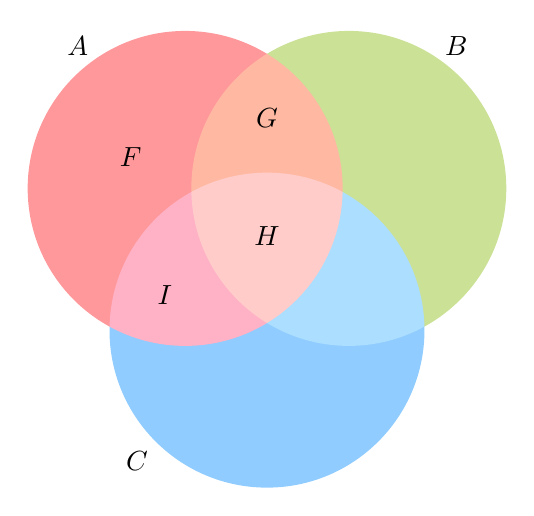
\begin{tikzpicture}
	\definecolor{vennred}{HTML}{ff989b}
	\definecolor{vennblue}{HTML}{90ccff}
	\definecolor{venngreen}{HTML}{cbe196}
	\begin{scope}[blend group = soft light]
		%						\fill[red!30!white!90]   ( 150:1.2) circle (2);
		\fill[vennred]   ( 150:1.2) circle (2);
		%						\fill[blue!30!white!90] (270:1.2) circle (2);
		\fill[vennblue] (270:1.2) circle (2);
		%						\fill[green!30!white!90]  (30:1.2) circle (2);
		\fill[venngreen]  (30:1.2) circle (2);
	\end{scope}
	\node at (135:3.4) {$ A $};
	\node at (45:3.4) {$ B $};
	\node at (240:3.3)	{$ C $};
	\node at ( 150:2)    {$ F $};
	\node at (90:1.5) 	{$ G $};
	\node at (210:1.5) 	{$ I $};
	\node [] {$ H $};
\end{tikzpicture}
\end{document}